\documentclass{article}
\usepackage{graphicx}
\usepackage{subcaption}
\graphicspath{{images/}}

\begin{document}

\title{TDS Data Processing}
\author{Yang Dai}
\maketitle

\section{Introduction}
There are several things we need to understand before we start processing the
TDS data. First, H\textsubscript{2} was found not only adsorbed on the front
surface of the crystal during beam dosing, but also the back of the
crystal. This has been a known issue, but expecially stands out in this set of
experiments possibly due to the high H\textsubscript{2} beam pressure (80 psi)
and long beam exposure time (300s). When dosing, the background pressure of
H\textsubscript{2} is at around $8\times 10^{-8}$ Torr. It is equivalent to ~24
L of H\textsubscript{2} background dose, which is too significant to be
ignored. To solve this problem, the Ni sample was prepared in such a way that
its front surface was covered by a thick layer of Au particles (QCM frequency
loss=250Hz). By doing so, the front face of the cyrtal should be completely
prevented from adsorbing any hydrogen. A TDS spectrum was then collected, which
we call \textit{background TDS}. The difference of the regular TDS and the
background TDS should be the amount of H\textsubscript{2} desorbed from the
front face of the Ni surface. However, this leads to another problem.

When comparing different TDS spectra, the Mass Spec sensitivity has to be taken
into account. The easiest way is to normalize all the TDS data to that of the
background TDS so that all the TDS spectra are comparable. To do this,  we
measured the mass spectrometer signal for a series of fixed background presure
of H\textsubscript{2}, allowing us to correct for any day-to-day variatinos in
mass spectrometer sensitivity due to factors such as multiplier gain.

\section{Data Processing}
\subsection{Step One-Obtain the Background TDS and sensitivity}
As mentioned above, the background TDS, as shown in Figure 1, was obtained for
the sample where its front surface was covered by a thick layer of Au
particles. Clearly, a substantial amount of H\textsubscript{2}  observed
between 200 K and 400 K should be attributed to the surafces other than the
front surface of the crystal.

A sensitivity experiment was performed at the end of the day. The mass
spectrometer siginal of H\textsubscript{2} was measured at different pressures,
as shown in Figure 2. The averaged counts and their corresponding pressures,
including the origin, were fitted using a linear regression model. The slope of
the fitted line is the sensitivity of the mass spectrometer on that day. The
same procedure was also followed for other TDS experiments as well. Sensitivity
experiment is usually done at the end of the day.

\begin{figure}[h]
\begin{subfigure}{0.5\textwidth}
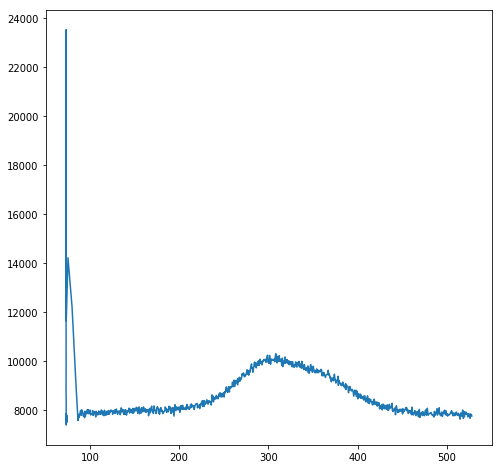
\includegraphics[width=0.9\linewidth, height=5cm]{background_tds.png}
\caption{}
\label{fig:subim1-a}
\end{subfigure}
\begin{subfigure}{0.5\textwidth}
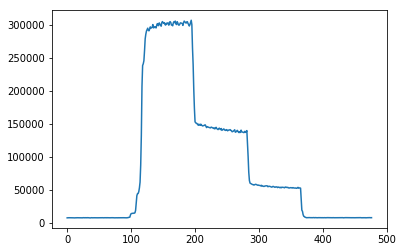
\includegraphics[width=0.9\linewidth, height=5cm]{sensitivity.png}
\caption{}
\label{fig:subim1-b}
\end{subfigure}
\begin{subfigure}{0.5\textwidth}
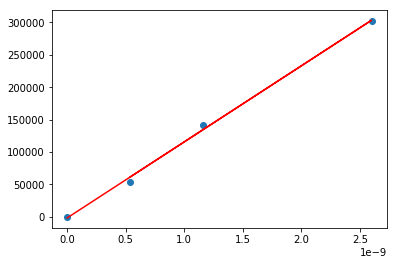
\includegraphics[width=0.9\linewidth, height=5cm]{sensitivity_regression.png}
\caption{}
\label{fig:subim1-c}
\end{subfigure}
\caption{a) H\textsubscript{2} background TDS taken for the Ni crystal whose
    surface was covered by a thick layer of Au particles. b) H\textsubscript{2}
    mass spectrometer signal vs. time at different background pressure. c) The
    fitted linear regression of the averaged counts against their corresponding
    pressure.}
\label{fig:image1}
\end{figure}

\subsection{Step Two-TDS Spectrum Preprocessing}
So far, we have done a series of TDS and CIRD experiments to discover the
nature of H\textsubscript{2} adsorption on NiAu alloy surface. Each set of
experiment is consisted of two TDS spectra, which are a reference TDS taken
before CIRD experiment, and a TDS taken after CIRD, a CIRD plot
(H\textsubscript{2} counts vs. time), and a sensitivity plot. The collected
data on Nov28 is taken as an example, shown in Figure 2.

Before normalizing a TDS spectrum, we preprocess the data first. Shortly after
the heating starts during a TDS experiment, the heating filament will relase a
substantial amount of H\textsubscript{2}, which can be detected by the Mass
Spectrometer, as shown in Figure 2a. We then remove this spike by eliminating
those datapoints before 95 K as shown in Figure 2b.

\begin{figure}[h]
\begin{subfigure}{0.5\textwidth}
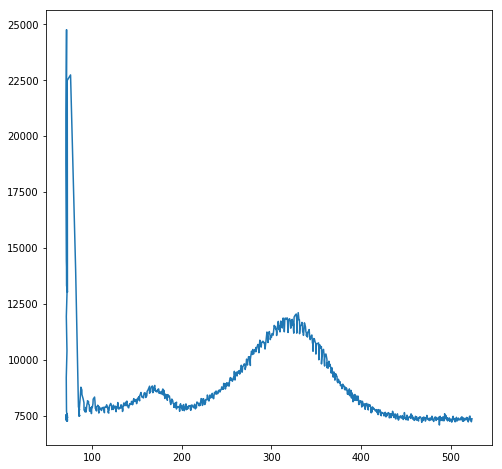
\includegraphics[width=0.9\linewidth, height=5cm]{tds_raw.png}
\caption{}
\label{fig:subim2-a}
\end{subfigure}
\begin{subfigure}{0.5\textwidth}
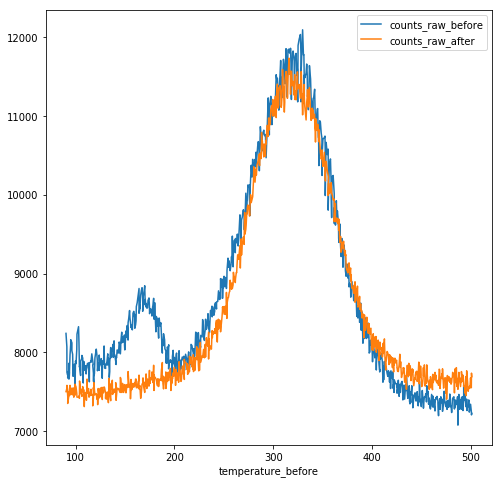
\includegraphics[width=0.9\linewidth, height=5cm]{spike_remove.png}
\caption{}
\label{fig:subim2-b}
\end{subfigure}
\begin{subfigure}{0.5\textwidth}
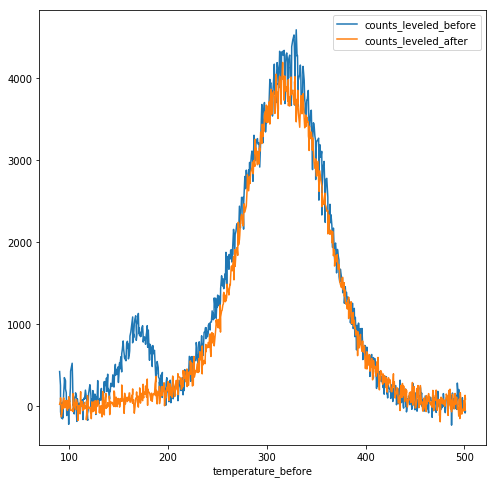
\includegraphics[width=0.9\linewidth, height=5cm]{leveled.png}
\caption{}
\label{fig:subim2-c}
\end{subfigure}
    \caption{a) a raw TDS spectra taken before CIRD experiment. b) TDS spectra
    taken before and after CIRD experiment. The spikes at the
    beginning of TDS experiments have been removed in both spectra.c) Both
    spectra have been leveled and the baseline has been moved to the x-axis.}
\label{fig:image2}
\end{figure}

When we carefully examine Figure 2b, a problem becomes apparent, \textit{i.e},
the difference of their baselines, which is due to the residual
H\textsubscript{2} during TDS experiments. This effect is especially dominat in
CIRD plot. To eliminate this effect, we collect10 datapoints at the beginning
and the end of the spectrum, and calculate the slope of the linear regression
of these datapoints, and use it to level the spectrum. In order to make the
comparison between TDS spectra easier, we further lower the baseline to 0.
Overall, after this adjustment, all the TDS spectra have the same baseline,
\textit{i.e}, the x-axis, as shown in Figure 2c.

\subsection{Step Three-Sensitivity Correction}
Now that all the TDS spectra, including the background TDS, have the same
baseline, in order to do the background subtraction, we need to correct the
sensitivity first, in other words, all TDS spectra should be normalized to the
sensitivity of the background TDS. To do this, we use the following equations:

$$Sensitivity\ Factor=\frac{Current\ Sensitivity}{Background\ Sensitivity}$$
$$Counts\_Corrected=\frac{Counts\_Original}{Sensitivity\ Factor}$$

Figure 3 shows the difference of two TDS spectra before and after sensitivity
correction. The sensitivity for the background TDS is $1.4754\times 10^{14}$,
and the sensitivity for the TDS that we are insterested in is $1.1723\times
10^{14}$. Because current sensitivity is less than that for the background TDS,
it means mass spectrometer is less sensitive as compared to when the background
was performed. As a result, after the sensitivity correction, the counts
become higher. Note that the baseline is still unchanged after sensitivity
correction because the baseline is at the x-axis, \textit{i.e}, 0.

\begin{figure}[h]
\centering
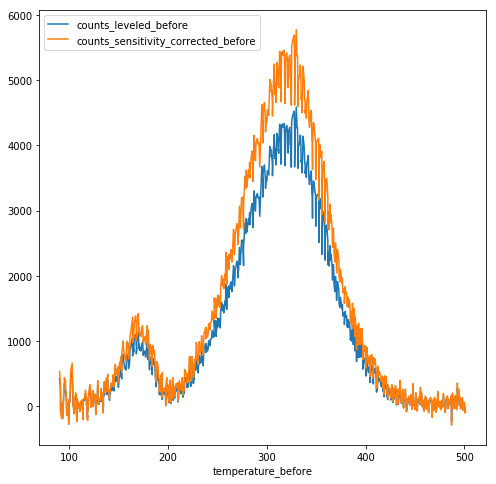
\includegraphics[width=0.6\linewidth, height=5cm]{sensitivity_correction.png}
\caption{TDS spectra before and after sensitivity correction.}
\label{fig:image3}
\end{figure}

\subsection{Step Four-Background Subtraction}
Up to this point, all the TDS spectra, including background TDS, are leveled,
and have the same baseline and sensitivity, so they are ready to do the
background subtraction. Figure 4 shows the difference of TDS spectra before and
after background subtraction for the TDS experiments done on Nov28.

\begin{figure}[h]
\begin{subfigure}{0.5\textwidth}
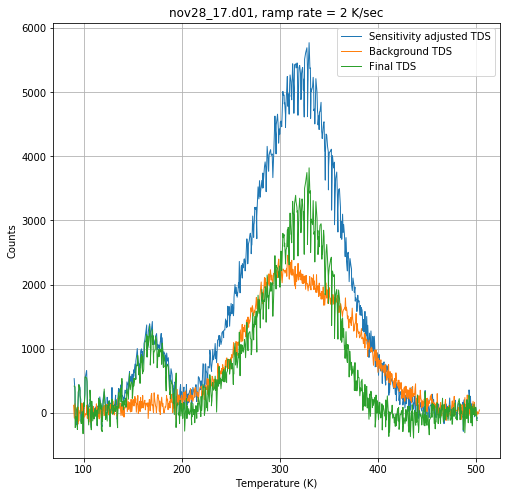
\includegraphics[width=0.9\linewidth,
    height=5cm]{background_subtraction_before.png}
\caption{}
\label{fig:subim4-a}
\end{subfigure}
\begin{subfigure}{0.5\textwidth}
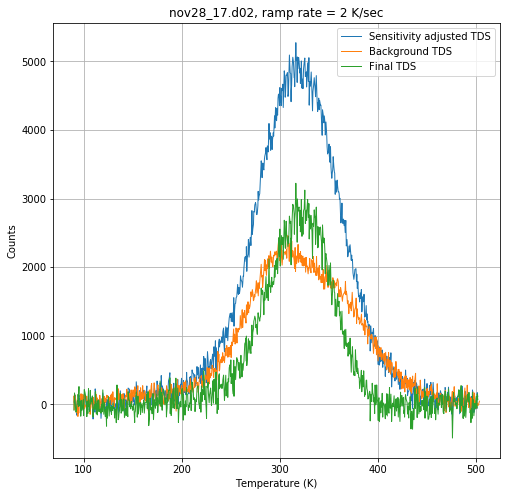
\includegraphics[width=0.9\linewidth,
    height=5cm]{background_subtraction_after.png}
\caption{}
\label{fig:subim4-b}
\end{subfigure}
    \caption{H\textsubscript{2} TDS spectra on AuNi alloy surface taken (a)
    before CIRD experiment (b) after CIRD experiment.}
\label{fig:image3}
\end{figure}

\section{Notes}
The whole process was automated with a program written in python. The program
will output a txt file that contains all the processed data and can be imported
into Igor for data visualization.

\end{document}
